\documentclass[tikz,border=12pt]{standalone}
\usepackage[utf8]{inputenc}
\usepackage[T1]{fontenc}
\usepackage{helvet}
\renewcommand{\familydefault}{\sfdefault}
\usetikzlibrary{arrows.meta,calc,fit,backgrounds}

\tikzset{
	inp/.style={draw=black, rounded corners=4pt, fill=gray!65, text=white,
		minimum width=1.7cm, minimum height=0.62cm, line width=0.6pt},
	hid/.style={draw=black, rounded corners=4pt, fill=gray!50,
		minimum width=1.7cm, minimum height=0.62cm, line width=0.6pt},
	outw/.style={draw=black, rounded corners=4pt, fill=gray!15, text=black,
		minimum width=1.7cm, minimum height=0.62cm, line width=0.6pt},
	focus/.style={draw=black, rounded corners=10pt, line width=0.9pt,
		inner xsep=9pt, inner ysep=10pt},
	rowlab/.style={anchor=east, font=\small},
	title/.style={font=\Large, anchor=east},
	note/.style={font=\bfseries\small, align=center},
	arr/.style={-{Stealth[length=2.4mm]}, line width=0.8pt},
}

\newcommand{\dx}{2.6}

\begin{document}
	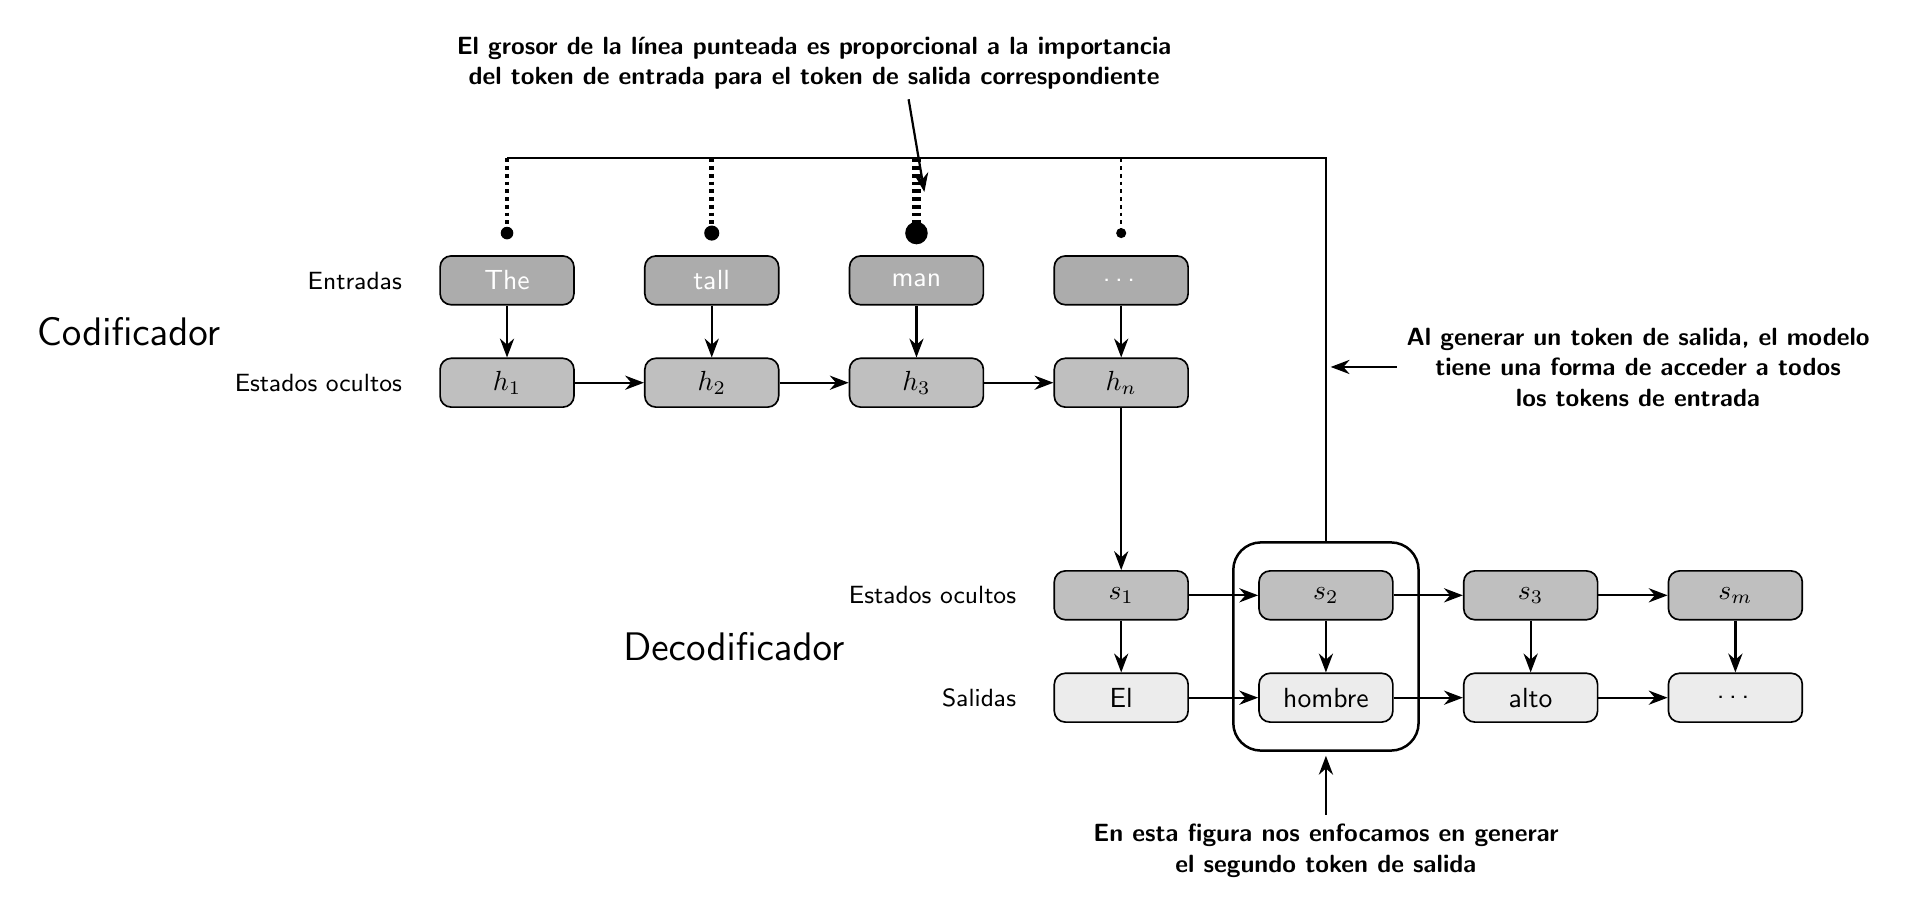
\begin{tikzpicture}
		
		%% ============================ Codificador (arriba) ============================
		\foreach \w [count=\i] in {The,tall,man,\dots}
		\node[inp] (x\i) at ({(\i-1)*\dx},0) {\w};
		\foreach \lab [count=\i] in {h_1,h_2,h_3,h_n}
		\node[hid] (h\i) at ({(\i-1)*\dx},-1.3) {$\lab$};
		
		\foreach \i in {1,...,4}
		\draw[arr] (x\i.south) -- (h\i.north);
		\foreach \i/\j in {1/2,2/3,3/4}
		\draw[arr] (h\i.east) -- (h\j.west);
		
		\node[rowlab] (lx) at ($(x1.west)+(-0.35,0)$) {Entradas};
		\node[rowlab] (lh) at ($(h1.west)+(-0.35,0)$) {Estados ocultos};
		\node[title] at ($(lh.west)!0.5!(lx.west)+(-0.4,0)$) {Codificador};
		
		%% =========================== Decodificador (abajo) ===========================
		\def\yd{-4.0}
		\foreach \lab [count=\i] in {s_1,s_2,s_3,s_m}
		\node[hid] (s\i) at ({(\i+2)*\dx},\yd) {$\lab$};
		\foreach \w [count=\i] in {El,hombre,alto,\dots}
		\node[outw] (y\i) at ({(\i+2)*\dx},\yd-1.3) {\w};
		
		\foreach \i in {1,...,4}
		\draw[arr] (s\i.south) -- (y\i.north);
		\foreach \i/\j in {1/2,2/3,3/4}
		\draw[arr] (s\i.east) -- (s\j.west);
		\foreach \i/\j in {1/2,2/3,3/4}
		\draw[arr] (y\i.east) -- (y\j.west);
		
		\node[rowlab] (ls) at ($(s1.west)+(-0.35,0)$) {Estados ocultos};
		\node[rowlab] (ly) at ($(y1.west)+(-0.35,0)$) {Salidas};
		\node[title] at ($(ls.west)!0.5!(ly.west)+(-0.4,0)$) {Decodificador};
		
		%% Último estado oculto del codificador -> primer estado del decodificador
		\draw[arr] (h4.south) -- (s1.north);
		
		%% Recuadro: generación del segundo token de salida
		\node[focus, fit=(s2)(y2)] (foc) {};
		
		%% ======================= Acceso a todos los tokens de entrada =======================
		% Pesos de atención (ilustrativos) para generar "hombre": man > tall > The > ...
		\def\ybus{1.55}
		\draw[line width=0.8pt] (x1.north |- 0,\ybus) -- (foc.north |- 0,\ybus) -- (foc.north);
		\foreach \i/\w in {1/0.15, 2/0.25, 3/0.55, 4/0.05}{
			\coordinate (d\i) at ($(x\i.north)+(0,0.28)$);
			\draw[line width={(0.6+5*\w)*1pt}, dash pattern=on 1.4pt off 1.4pt]
			(x\i.north |- 0,\ybus) -- (d\i);
			\fill (d\i) circle[radius={(1.6+4.5*\w)*1pt}];
		}
		
		%% =============================== Anotaciones ================================
		\node[note, anchor=south] (n1) at ($(x3.north |- 0,\ybus)+(-1.3,0.75)$)
		{El grosor de la línea punteada es proporcional a la importancia\\
			del token de entrada para el token de salida correspondiente};
		\draw[arr] ($(n1.south)+(1.2,0)$) -- ($(x3.north |- 0,\ybus)!0.45!(d3)+(0.1,0)$);
		
		\node[note, anchor=west] (n2) at ($(foc.north |- h4)+(0.9,0.2)$)
		{Al generar un token de salida, el modelo\\
			tiene una forma de acceder a todos\\
			los tokens de entrada};
		\draw[arr] (n2.west) -- ($(foc.north |- n2.west)+(0.06,0)$);
		
		\node[note, anchor=north] (n3) at ($(foc.south)+(0,-0.8)$)
		{En esta figura nos enfocamos en generar\\el segundo token de salida};
		\draw[arr] (n3.north) -- ($(foc.south)+(0,-0.05)$);
		
	\end{tikzpicture}
\end{document}